% \iffalse meta-comment
%
% rubikpatterns.dtx
%
% version 5.0
%
% Authors: RWD Nickalls (dick@nickalls.org) 
%        and Apostolos Syropoulos (asyropoulos@yahoo.com)
%
% Copyright   25 February 2018  RWD Nickalls + A Syropoulos
%
% This work may be distributed and/or modified under the
% conditions of the LaTeX Project Public License, either
% version 1.3c of this license or (at your option) any
% later version. The latest version of this licence is in 
%
%       http://www.latex-project.org/lppl.txt
%
%<*readme>
%
% The rubikpatterns package provides a collection of LaTeX commands and macros 
% for the typesetting of Rubik cube configurations and rotation 
% sequences using the TikZ graphic language.
%
% Please report errors or suggestions for improvement to
%
%         Dick Nickalls or Apostolos Syropoulos
%
% This package requires the basic TikZ package to be loaded already
%</readme>
%
%<*driver>
\listfiles
\documentclass{ltxdoc}
\IfFileExists{rubikpatterns.sty}{\usepackage{rubikpatterns}}{%
    \GenericWarning{rubikpatterns.dtx}{Package file rubikpatterns.sty not found.
    Documentation will be messed up!^^J
    (Generate rubikpatterns.sty by (La)TeXing rubikpatterns.ins, and then^^J
    process rubikpatterns.dtx again)^^J}\stop
}%
\pagestyle{myheadings}
\markright{\texttt{rubikpatterns} \ \ (Rubik bundle v5.0, 2018) \ \ \texttt{www.ctan.org/pkg/rubik}}
\usepackage{ifpdf}
\usepackage{url,path}  %% for references and paths
\usepackage{graphicx}  %% for the two pdf figs
\usepackage{hypdoc}    %% for pdf bookmarks + hyperref documenting of packages
%%\OnlyDescription
\EnableCrossrefs
\PageIndex
\CodelineIndex
\CodelineNumbered
\RecordChanges
\setcounter{StandardModuleDepth}{1}
\begin{document}
  \DocInput{rubikpatterns.dtx}
  \PrintChanges
  \PrintIndex
\end{document}
%</driver>
% \fi
%
%
% 
%%% \CheckSum{187}
%
%%% \CharacterTable
%%  {Upper-case    \A\B\C\D\E\F\G\H\I\J\K\L\M\N\O\P\Q\R\S\T\U\V\W\X\Y\Z
%%   Lower-case    \a\b\c\d\e\f\g\h\i\j\k\l\m\n\o\p\q\r\s\t\u\v\w\x\y\z
%%   Digits        \0\1\2\3\4\5\6\7\8\9
%%   Exclamation   \!     Double quote  \"     Hash (number) \#
%%   Dollar        \$     Percent       \%     Ampersand     \&
%%   Acute accent  \'     Left paren    \(     Right paren   \)
%%   Asterisk      \*     Plus          \+     Comma         \,
%%   Minus         \-     Point         \.     Solidus       \/
%%   Colon         \:     Semicolon     \;     Less than     \<
%%   Equals        \=     Greater than  \>     Question mark \?
%%   Commercial at \@     Left bracket  \[     Backslash     \\
%%   Right bracket \]     Circumflex    \^     Underscore    \_
%%   Grave accent  \`     Left brace    \{     Vertical bar  \|
%%   Right brace   \}     Tilde         \~}
%
%
%
% \title{%
%       \ifpdf\pdfbookmark[1]{Title}{Title}\else\fi%
%       The \textsc{rubikpatterns} package}
%
% \author{
%      RWD Nickalls (dick@nickalls.org) \\
%     A Syropoulos (asyropoulos@yahoo.com)
%       }
%  \date{This file describes version \RPfileversion\ (\RPfiledate)\\
%  \texttt{www.ctan.org/pkg/rubik}}
%  \maketitle
%
%  \begin{abstract}
%  The \rubikpatterns\ package is a small data-base of well-known named 
%  Rubik patterns and associated rotation sequences, for use  in conjunction 
%  with the other Rubik `bundle' packages. 
%  \end{abstract}
%
%
%  \tableofcontents
%
% \pagebreak
%
% \section{Introduction}
%
%  The \textsc{rubikpatterns}  package is a small a data-base of well-known  Rubik 
%  rotation sequences  for use  in  conjunction with the Rubik bundle packages. 
%  These rotation sequences, which are well-known and  widely available, 
%  were  sourced from the Rubik-related
%  websites  of Reid M and Kociemba H (see References for URLs). 
%
%
%
%      \section{Requirements}
%
%  The \textsc{rubikpatterns} package requires (a)~the TikZ package, since it makes  
%  use  of the TikZ picture environment, (b)~the \textsc{rubikcube} package, and 
%  (c)~the \textsc{rubikrotation} package, since it uses
%  the Perl program \texttt{rubikrotation.pl}.
%  The \verb!TikZ! package must be loaded \textit{before} the \textsc{rubikcube}  package.
%  The \textsc{rubikrotation}  package  requires  Perl to be installed.
%
%
%
%   \section{Installation}
%
%
% The Rubik bundle consists of the four packages \textsc{rubikcube}, \textsc{rubikrotation},
% \textsc{rubikpatterns} and  \textsc{rubiktwocube}.
%
% Here we describe only the installation of the \textsc{rubikpatterns} package, 
% which  consists of the  following files:
%\begin{quote}
% \begin{verbatim}
% rubikpatterns.ins
% rubikpatterns.dtx
% rubikpatterns.pdf       --this document
% rubikpatternsLIST.tex
% rubikpatternsLIST.pdf   --a graphic list of all patterns in this package  
% rubikpatterns-doc-figA.pdf
%\end{verbatim}
%\end{quote}
% The package documentation is the file \texttt{rubikpatterns.pdf}.
%  The  style option \texttt{rubikpatterns.sty} is generated  by  running (pdf)\LaTeX\ on  
% the file \texttt{rubikpatterns.ins}  as follows:
%\begin{quote}
%\begin{verbatim}
%   pdflatex  rubikpatterns.ins 
%\end{verbatim}
%\end{quote}
% The documentation file (\texttt{rubikpatterns.pdf}) is then generated using the following 
% sequence of steps\,\footnote{Since the documentation includes a complicated indexing 
% system as well a \textsc{pdf} index and hyperef links (the package \texttt{hypdoc}
%  is used), then a lot of pdflatex runs are required. Prior to the first run it is
% a good idea to delete any relevant \texttt{.toc}, \texttt{.aux}, \texttt{.out} files.}:
%\begin{quote}
% \begin{verbatim}
%  pdflatex    rubikpatterns.dtx
%  pdflatex    rubikpatterns.dtx
%  makeindex -s gind.ist  rubikpatterns
%  makeindex -s gglo.ist -o rubikpatterns.gls  rubikpatterns.glo
%  pdflatex    rubikpatterns.dtx
%  pdflatex    rubikpatterns.dtx
%\end{verbatim}
%\end{quote}
%
%
% 
%  \subsection{Placing the files}
% \label{sec:placingfiles}
%
% Place the files either in a working directory, or where your system 
% will find them, e.g.,~in your \texttt{/texmf-local/} directory tree. 
% For example, on a Linux platform with a standard \TeX\ Directory Structure (TDS), then:
%
%\medskip
%{\noindent}*.sty  $\rightarrow$  \texttt{/usr/local/texlive/texmf-local/tex/latex/rubik/}
%{\newline}*.pdf  $\rightarrow$  \texttt{/usr/local/texlive/texmf-local/doc/rubik/}
%
%\medskip
%
%\medskip
%{\noindent}\textsc{file database}:\ \ Finally, (depending on your system) update the 
% \TeX\ file database. 
% For example, on a Linux platform  this is achieved using the \texttt{texhash} command.
%
% 
%  \subsection{The  rubikpatternsLIST file}
%

% Note that the package includes a  `rubikpatternsLIST' file (\texttt{rubikpatternsLIST.pdf}), 
% as well  as the source file  (\texttt{rubikpatternsLIST.tex}), and
%  associated  \texttt{.sh} (Linux) and \texttt{.bat} (Microsoft) batch 
% files, which can be used to facilitate processing the  source \texttt{.tex} file. 
% The file \texttt{rubikpatternsLIST.pdf} showcases the  Rubik cube 
% patterns made available in this package.
%
% Note that should you need to generate the file \texttt{rubikpatternsLIST.pdf} 
% from the  source file (\texttt{rubikpatternsLIST.tex}) you will require
% the \textsc{rubikcube} and  \textsc{rubikrotation} packages to be installed,
%  and will also need to use the \verb!--shell-escape! command-line 
% option  (see Section~\ref{sec:rubikrotation} for details). 
%
%
%
%
%
%       \subsection{Usage}
% \label{sec:usage}
% Load the  packages \textsc{rubikcube}, 
%  \textsc{rubikrotation} and \textsc{rubikpatterns} in the \TeX\ file preamble  \textit{after} loading 
% the TikZ package; for example, as follows: 
%\begin{quote}
% \begin{verbatim}
% \usepackage{tikz}
% \usepackage{rubikcube,rubikrotation,rubikpatterns}
%\end{verbatim}
%\end{quote}
% Since the sequence macros made available  by this package are accessed using commands 
% provided by the \textsc{rubikcube} and \textsc{rubikrotation} packages, please read the 
% documentation of these  packages.
%
%
% 
%   \section{Rubik patterns}
%
% A Rubik pattern  is the configuration generated by a sequence of rotations 
% (or `moves') from some initial starting configuration (typically a `solved' 
% configuration). For example, `sixspot' is a well known pattern  generated  
% from a solved Rubik cube by the  rotation sequence  
% \texttt{U,Dp,R,Lp,F,Bp,U,Dp}, as follows:
%
% \bigskip
%
% \noindent\begin{minipage}{\textwidth}
% \centering
% \ifpdf
%   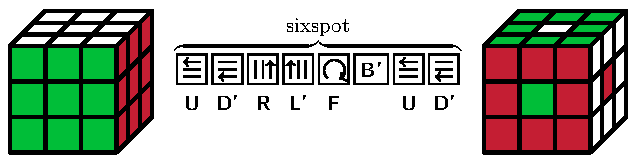
\includegraphics[height=3cm]{rubikpatterns-doc-figA.pdf}
% \else
% \fi
% \end{minipage}
%
% \bigskip
%
% {\noindent}The code for the above image is as follows:
%
%\begin{verbatim}
% \noindent\hfil%
% \RubikCubeSolvedWB% 
% \ShowCube{2.4cm}{0.6}{\DrawRubikCubeRU}%
% \RubikRotation{\SixSpot}%
% \quad\SequenceBraceA{sixspot}{\ShowSequence{}{\Rubik}{\SequenceLong}}\quad%
% \ShowCube{2.4cm}{0.6}{\DrawRubikCubeRU}%
% \hfil%
%\end{verbatim}
%
% \bigskip
%
% Note that the  appearance of a pattern generated by  a given 
% rotation sequence is, of course, sensitive  to (a)~the particular colour 
% configuration of the solved cube used, and (b)~the initial  orientation of 
% the Rubik cube.
% 
% 
% Consequently the appearance generated  by a given sequence
% may appear  slightly different from 
% that on some websites, although the  colour configuration (pattern's \textit{geometry})   
% will, of course, be the same  (isomorphic). You may therefore need 
% to adjust the pre- (and possibly the post-)  x,y,z rotations in 
% order to obtain  a particular configuration as displayed elsewhere.
%
%
%  \subsection{Sequence macros}
%
% Each of the  rotation sequences of `patterns'  made available by the 
% \textsc{rubikpatterns} package is defined in  the file \texttt{rubikpatterns.sty}  
% in the following  compact macro form.
% For~example, the rotation sequence associated with the pattern known 
% as `SixSpot' (shown in the figure above) is defined as follows:
%\begin{verbatim}
%\newcommand{\SixSpot}{[SixSpot],U,Dp,R,Lp,F,Bp,U,Dp,<(8q*, 8f*)>}
%\newcommand{\sixspot}{\SixSpot}
%\end{verbatim}
% The macro name is \verb!\SixSpot! (the lower-case version \verb!\sixspot! can also be used). 
% Note that the second argument which 
% includes the  rotation sequence, also includes the pattern name in 
% square brackets \verb![SixSpot]!  as the first element in the sequence.
% Additional metadata (held by the macro \verb!\SequenceInfo!) is appended 
% in angle brackets (separated by a comma) as follows: \verb!<(8q*, 8f*)>!.
% For  details see  the \textsc{rubikrotation} package documentation.
%
%
%
%   \subsection{List of macros}
%
% The following is a list of the macro names of all the Rubik patterns supplied by
% the \textsc{rubikpatterns} package.  Note that for convenience each macro-name listed
% has an equivalent lower-case version. See the companion file \texttt{rubikpatternsLIST.pdf}
% for a detailed list  showing  each pattern  and its associated 
% sequence\,\footnote{We show all these images in a separate
% file (\texttt{rubikpatternsLIST.pdf}) purely because  generating them requires 
% using the \LaTeX\ command-line  option \texttt{--shell-escape} in conjunction 
% with the \textsc{rubikrotation} package.}. 
%
%  All the pattern names encoded here (as macros) are  well-known and widely available. 
% However, some pattern names have been slightly modified
% in order to avoid spaces and to keep them as similar to the original as possible.
% On finding different sequences which generate the same pattern, then the  
% shortest  sequence has been selected   (they can be readily distinguished by their metadata).
% 
% Finally, we note that there is a serious need for a standardised one-word nomenclature 
% in order to  avoid confusion, and to facilitate computerisation and an electronic database.
% Such a notation also needs to accommodate  those sequence variations which generate the same pattern.
% We welcome suggestions and/or help for improvement.

%
%\begin{verbatim}
%  \PonsAsinorum
%  \CheckerboardsThree
%  \CheckerboardsSix
%  \Stripes
%  \CubeInCube
%  \CubeInCubeInCube
%  \ChristmasCross
%  \PlummersCross
%  \Anaconda
%  \Python
%  \BlackMamba
%  \GreenMamba
%  \FemaleRattlesnake
%  \MaleRattlesnake
%  \FemaleBoa
%  \MaleBoa
%  \FourSpot
%  \SixSpot
%  \OrthogonalBars
%  \SixTs
%  \SixTwoOne
%  \ExchangedPeaks
%  \TwoTwistedPeaks
%  \FourTwistedPeaks
%  \ExchangedChickenFeet
%  \TwistedChickenFeet
%  \ExchangedRings
%  \TwistedRings
%  \EdgeHexagonTwo
%  \EdgeHexagonThree
%  \TomParksPattern
%  \RonsCubeInCube
%  \TwistedDuckFeet
%  \ExchangedDuckFeet
%  \Superflip
%\end{verbatim}
%
% Note that  the particular  superflip sequence made available by this package 
% (shown in \texttt{rubikpatternsLIST.pdf}) is due to  Reid (1995), and is detailed 
% on the Kociemba webpage  \texttt{http://www.kociemba.org/math/oh.htm}. Indeed, this was the 
% first sequence to define the `20-move' (HTM) upper boundary for solving a Rubik cube 
% (see  Rokicki \textit{et~al.}, 2013). 
%
% The superflip configuration is also significant  since it is its own inverse. 
% For example, the following two \verb!\RubikRotation! commands will generate the same 
% configuration (starting from a solved cube):
%\begin{verbatim}
% \RubikRotation{\superflip}
% \RubikRotation{\superflip,<inverse>}
%\end{verbatim}
% This property  is shown as  one of the examples in the Rubik bundle  file \texttt{rubikexamples.pdf}.
%
%
%
%     \section{Change history}
%
% \begin{itemize}
%
% \item Version 4.0 (March 2017)
%
% --- First release of this package.
%
% \end{itemize}
%
%
%
%   \section{References}
%     \label{sec:references}
%
%\begin{itemize}
%
% \item Fridrich website (Fridrich J). 
% See the `Pretty patterns'  webpage \url{http://www.ws.binghamton.edu/fridrich/ptrns.html}
%
% \item  Kociemba website (Kociemba H).  \url{http://www.kociemba.org/cube.htm}
% {\newline}---for superflip see: \url{http://www.kociemba.org/math/oh.htm}
%
% \item Randelshofer website (Randelshofer W).  Pretty patterns. 
% \url{http://www.randelshofer.ch/rubik/patterns/U080.01.html}
%
% \item Reid M. \  Patterns.  \url{http://www.cflmath.com/Rubik/patterns.html}
%
% \item Reid M. (1995). Superflip requires 20 face turns. (January 1995) 
%   \url{http://www.math.ucf.edu/~reid/Rubik/CubeLovers/} 
%  (see Section~\ref{sec:superflip})  
% {\newline}[cited from Rokicki \textit{et~al.}, 2013]. 
% {\newline}(Note: easier to use is the following html indexed version of the 
% archive of the Cube-Lovers usenet group (1982--1997)  
% \url{http://www.math.rwth-aachen.de/~Martin.Schoenert/Cube-Lovers/})
%
%  \item Rokicki T, Kociemba H, Davidson M and Dethridge J (2013). The diameter of the Rubik's 
%  cube is twenty.  \textit{SIAM.\ J.\ Discrete Math.}, \textbf{27}, 1082--1105. 
%   \url{http://tomas.rokicki.com/rubik20.pdf}
%
%\end{itemize}
% 
%
%
%
% ^^A ==================================================
% \StopEventually{\PrintIndex}
%
%
%
%        \section[The code]{The code (\texttt{rubikpatterns.sty})} 
%
% 
%   \subsection{Package heading}
%   \label{sec:CodePackageHeading}
%
%    \begin{macrocode}
%<*rubikpatterns>
\def\RPfileversion{5.0}%
\def\RPfiledate{2018/02/25}%  25 February 2018
\NeedsTeXFormat{LaTeX2e}
\ProvidesPackage{rubikpatterns}[\RPfiledate\space (v\RPfileversion)]
%    \end{macrocode}
%
%
%    \begin{macro}{\rubikpatterns}
% First we create a suitable logo
%    \begin{macrocode}
\newcommand{\rubikpatterns}{\textsc{rubikpatterns}}
%    \end{macrocode}
%    \end{macro}
%
%   \subsection{Patterns}
%   \label{sec:patternscode}
%
%
%
%
%  \subsubsection{Superflip}
%   \label{sec:superflip}
%
% This particular superflip sequence is from the Kociemba website (his Oh webpage). 
% It is due to  Reid (1995).
%  \begin{macrocode}
\newcommand{\Superflip}{[Superflip],Dp,R2,Fp,D2,F2,U2,Lp,R,Dp,R2,B,F,Rp,%
U2,Lp,F2,Rp,U2,Rp,Up,<(20f*)>}%
\newcommand{\superflip}{\Superflip}
%    \end{macrocode}
%
%
%  \subsubsection{Reid data}
%
% These named sequences are derived from the Reid website. 
%  \begin{macrocode}
\newcommand{\PonsAsinorum}{[PonsAsinorum],F2,B2,R2,L2,U2,D2,%
   <(12q*, 6f*)>}%
\newcommand{\ponsasinorum}{\PonsAsinorum}%
\newcommand{\CheckerboardsThree}%
   {[CheckerboardsThree],F,B2,Rp,D2,B,R,U,Dp,R,Lp,Dp,Fp,R2,D,F2,Bp,%
   <(20q*, 16f*), order 3>}%  
\newcommand{\checkerboardsthree}{\CheckerboardsThree}%
\newcommand{\CheckerboardsSix}%
   {[CheckerboardsSix],R2,L2,U,B,L2,Dp,F,B2,R,Lp,Fp,B,R,D,F2,Lp,Up,%
   <(17f*, 22q), order 6>}%  
\newcommand{\checkerboardssix}{\CheckerboardsSix}%
\newcommand{\Stripes}{[Stripes],F,U,F,R,L2,B,Dp,R,D2,L,Dp,B,R2,L,F,U,F,%
   <(20q*, 17f*)>}%  
\newcommand{\stripes}{\Stripes}%
\newcommand{\CubeInCube}{[CubeInCube],F,L,F,Up,R,U,F2,L2,Up,Lp,B,Dp,Bp,L2,U,%
   <(18q*, 15f*)>}%  
\newcommand{\cubeincube}{\CubeInCube}%
\newcommand{\CubeInCubeInCube}%
   {[CubeInCubeInCube],Fp,U,Bp,Rp,U,F2,U2,Fp,Up,F,U2,D,Bp,Dp,R2,B2,Up,%
   <(17f*, 22q)>}%  
\newcommand{\cubeincubeincube}{\CubeInCubeInCube}%
\newcommand{\ChristmasCross}{[ChristmasCross],U,F,Bp,L2,U2,L2,Fp,B,U2,L2,U,%
   <(16q*, 11f*)>}%  
\newcommand{\christmascross}{\ChristmasCross}%
\newcommand{\PlummersCross}%
   {[PlummersCross],R2,Lp,D,F2,Rp,Dp,Rp,L,Up,D,R,D,B2,Rp,U,D2,%
   <(20q*, 16f*)>}%  
\newcommand{\plummerscross}{\PlummersCross}%
\newcommand{\Anaconda}{[Anaconda],L,U,Bp,Up,R,Lp,B,Rp,F,Bp,D,R,Dp,Fp,%
   <(14q*, 14f*)>}%  
\newcommand{\anaconda}{\Anaconda}%
\newcommand{\Python}{[Python],F2,Rp,Bp,U,Rp,L,Fp,L,Fp,B,Dp,R,B,L2,%
   <(16q*, 14f*)>}%  
\newcommand{\python}{\Python}%
\newcommand{\BlackMamba}{[BlackMamba],R,D,L,Fp,R,Lp,D,Rp,U,Dp,B,Up,Rp,Dp,%
   <(14q*, 14f*)>}%  
\newcommand{\blackmamba}{\BlackMamba}%
\newcommand{\GreenMamba}{[GreenMamba],R,D,R,F,Rp,Fp,B,D,Rp,Up,Bp,U,D2,%
   <(14q*, 13f*)>}%    
\newcommand{\greenmamba}{\GreenMamba}%
\newcommand{\FemaleRattlesnake}%
   {[FemaleRattlesnake],U2,Dp,L2,D,B,U,Bp,Rp,L2,U2,F,Up,F,R,%
   <(18q*, 14f*)>}%  
\newcommand{\femalerattlesnake}{\FemaleRattlesnake}%
\newcommand{\MaleRattlesnake}%
   {[MaleRattlesnake],Rp,Fp,U,Fp,U2,R,L2,B,Up,Bp,Dp,L2,U2,D,%
   <(18q*, 14f*)>}%  
\newcommand{\malerattlesnake}{\MaleRattlesnake}%
\newcommand{\FemaleBoa}{[FemaleBoa],R,Up,R2,U2,F,D2,R2,Up,Dp,R,Dp,Fp,%
   <(16q*, 12f*)>}%  
\newcommand{\femaleboa}{\FemaleBoa}%
\newcommand{\MaleBoa}{[MaleBoa],F,D,Rp,U,D,R2,D2,Fp,U2,R2,U,Rp,%
   <(16q*, 12f*)>}%  
\newcommand{\maleboa}{\MaleBoa}%
\newcommand{\FourSpot}{[FourSpot],F2,B2,U,Dp,R2,L2,U,Dp,%
   <(12q*, 8f*)>}%  
\newcommand{\fourspot}{\FourSpot}%
\newcommand{\SixSpot}{[SixSpot],U,Dp,R,Lp,F,Bp,U,Dp,%
   <(8q*, 8f*)>}%  
\newcommand{\sixspot}{\SixSpot}%
\newcommand{\OrthogonalBars}%
   {[OrthogonalBars],F,Rp,U,L,Fp,Lp,F,Up,R,U,Lp,Up,L,Fp,%
   <(14q*, 14f*)>}%  
\newcommand{\orthogonalbars}{\OrthogonalBars}%
\newcommand{\SixTs}{[SixTs],F2,R2,U2,Fp,B,D2,L2,F,B,%
   <(14q*, 9f*)>}% 
\newcommand{\sixts}{\SixTs}%
\newcommand{\SixTwoOne}{[SixTwoOne],U,B2,D2,L,Bp,Lp,Up,Lp,B,D2,B2,%
   <(15q*, 11f*)>}%  
\newcommand{\sixtwoone}{\SixTwoOne}%
\newcommand{\ExchangedPeaks}%
   {[ExchangedPeaks],F2,R2,D,R2,U,D,F2,Dp,Rp,Dp,F,L2,Fp,D,R,Up,%
   <(16f*, 21q)>}%  
\newcommand{\exchangedpeaks}{\ExchangedPeaks}%
\newcommand{\TwoTwistedPeaks}%
   {[TwoTwistedPeaks],F,D2,B,R,Bp,Lp,F,Dp,L2,F2,R,Fp,Rp,F2,Lp,Fp,%
   <(16f*, 20q)>}%
\newcommand{\twotwistedpeaks}{\TwoTwistedPeaks}%
\newcommand{\FourTwistedPeaks}%
   {[FourTwistedPeaks],Up,D,B,Rp,F,R,Bp,Lp,Fp,B,L,F,Rp,Bp,R,Fp,Up,D,%
   <(18q*, 18f*)>}%
\newcommand{\fourtwistedpeaks}{\FourTwistedPeaks}%
\newcommand{\ExchangedChickenFeet}%
   {[ExchangedChickenFeet],F,Lp,Dp,Bp,L,F,U,Fp,Dp,F,L2,Bp,Rp,U,L2,Dp,F,%
   <(19q*, 17f*)>}%
\newcommand{\exchangedchickenfeet}{\ExchangedChickenFeet}%
\newcommand{\TwistedChickenFeet}%
   {[TwistedChickenFeet],F,Lp,D,Fp,Up,B,U,F,Up,F,Rp,F2,L,Up,Rp,D2,%
   <(18q*, 16f*)>}%
\newcommand{\twistedchickenfeet}{\TwistedChickenFeet}%
\newcommand{\ExchangedRings}%
   {[ExchangedRings],F,U,Dp,Lp,B2,L,Up,D,F,U,R2,L2,Up,L2,F2,%
   <(15f*, 20q)>}%
\newcommand{\exchangedrings}{\ExchangedRings}%
\newcommand{\TwistedRings}%
   {[TwistedRings],F,D,Fp,D2,Lp,Bp,U,L,D,R,U,Lp,Fp,U,L,U2,%
   <(18q*, 16f*)>}%
\newcommand{\twistedrings}{\TwistedRings}%
\newcommand{\EdgeHexagonTwo}%
   {[EdgeHexagonTwo],U,B2,Up,Fp,Up,D,Lp,D2,L,U,Dp,F,Dp,L2,B2,Dp,%
   <(20q*, 16f*) order2>}% 
\newcommand{\edgehexagontwo}{\EdgeHexagonTwo}%
\newcommand{\EdgeHexagonThree}%
   {[EdgeHexagonThree],F,L,B,U,L,F2,B2,Rp,F2,B2,Up,Bp,Lp,Fp,%
   <(14f*, 18q) order 3>}%
\newcommand{\edgehexagonthree}{\EdgeHexagonThree}%
\newcommand{\TomParksPattern}%
   {[TomParksPattern],L,U,F2,R,Lp,U2,Bp,U,D,B2,L,F,Bp,Rp,L,Fp,R,%
   <(20q*, 17f*)>}%
\newcommand{\tomparkspattern}{\TomParksPattern}%
\newcommand{\RonsCubeInCube}%
   {[RonsCubeInCube],L2,D2,Lp,D2,B2,L2,B2,Lp,D2,L2,B2,Lp,B2,%
   <(13f*, 23q)>}%
\newcommand{\ronscubeincube}{\RonsCubeInCube}%
\newcommand{\TwistedDuckFeet}%
   {[TwistedDuckFeet],F,Rp,B,R,U,Fp,Lp,Fp,U2,Lp,Up,D2,B,Dp,F,Bp,U2,%
   <(20q*, 17f*)>}%
\newcommand{\twistedduckfeet}{\TwistedDuckFeet}%
\newcommand{\ExchangedDuckFeet}%
   {[ExchangedDuckFeet],U,F,R2,Fp,Dp,R,U,B2,U2,Fp,R2,F,D,B2,R,Bp,%
   <(21q*, 16f*)>}%
\newcommand{\exchangedduckfeet}{\ExchangedDuckFeet}%
%    \end{macrocode}
% --------------------------
%    End of this package
% --------------------------
%    \begin{macrocode}
%</rubikpatterns>
%    \end{macrocode}
%
%
%
%
% \Finale
%
\endinput





